\documentclass[12pt,twoside]{article}
\usepackage{bokGalil}
\usepackage{lscape}
\usepackage{stix}
\begin{document}
\hypersetup{
   pdfauthor     = {P. N. Daly},
   pdfsubject    = {90Prime Software and Hardware Guide}
   pdftitle      = {90Prime Software and Hardware Guide}
   pdfkeywords   = {90Prime Software and Hardware Guide}
   }
\fancyhead[CE]{P.\ N.\ Daly}
\fancyhead[CO]{90Prime Software and Hardware Guide}
\title{90Prime Software and Hardware Guide}
\author{P.\ N.\ Daly}
\affil{Mountain Operations, Steward Observatory\altaffilmark{1} \\
933 N.\ Cherry Avenue, Tucson AZ 85719, U S A}
\altaffiltext{1}{
Steward Observatory is the research arm of the Department of Astronomy at the University of Arizona (UArizona). 
Its offices are located on the UArizona campus in Tucson, Arizona (US). Established in 1916, the first telescope 
and building were formally dedicated on April 23, 1923. It now operates, or is a partner in telescopes at five 
mountain-top locations in Arizona, one in New Mexico, one in Hawaii, and one in Chile. It has provided instruments 
for three different space telescopes and numerous terrestrial ones. Steward also has one of the few facilities in 
the world that can cast and figure the very large primary mirrors used in telescopes built in the early 21st century.}
\email{(520) 621-3648, pndaly@arizona.edu}
\begin{abstract}
This document describes the new software and hardware systems to support the upgraded 90Prime imager at 
the Bok 90-inch telescope. \\

\noindent \emph{Document revision date 20250408. Last author: Phil Daly (pndaly@arizona.edu).} \\
\end{abstract}

\tableofcontents
\listoffigures
\listoftables

\newpage
\section{Quick Start}
\label{quickstart}

\noindent To start the system, execute the following if operating on \sfmagenta{bonsai (10.30.1.7)}\footnote{If running from
\sfmagenta{banzai} (10.30.1.8), the command is: \emteal{ssh -XY primefocus@banzai}}: \\

\emteal{ssh -XY primefocus@bonsai}

\emteal{cd /home/primefocus/bokGalil}

\emteal{source \hspace{1mm} etc/bokGalil.sh \hspace{1mm} \$(pwd) \hspace{1mm} gui}\footnote{
  You can also replace the \emph{\$(pwd)} syntax with the `backward apostrophe' syntax: 
  \emph{{\small $^\backprime$}~pwd~{\small $^\backprime$}}. The `backward apostrophe' is often 
  located at the top-left of the keyboard sharing the `$\sim$' key below the {\sc esc} key.
  However, this syntax only works in the /home/primefocus/bokGalil sub-directory. From \emph{any} location, 
  use the full command syntax: \emph{source \hspace{1mm} /home/primefocus/bokGalil/etc/bokGalil.sh \hspace{1mm} /home/primefocus/bokGalil \hspace{1mm} gui}.} \\

\noindent Allow the interface shown in Figure~\ref{boktcl} to appear and press the \emteal{start} button. The last element
to appear---indicating that startup is complete---is a \emph{ds9} window  Then choose an appropriate web interface as shown 
in Figure~\ref{bokgui}: \\

\ttblue{http://10.30.1.7:5905} for astronomers, or

\ttblue{http://10.30.1.7:5905/indi} for engineers. \\

\begin{figure}[!h]
 \centering
 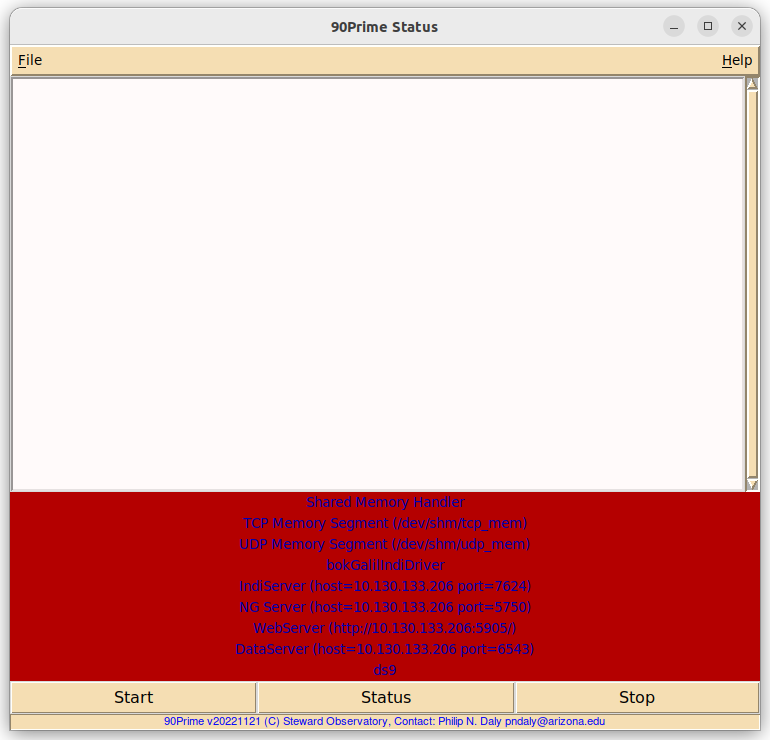
\includegraphics[width=0.4\linewidth]{bokSplashOff.png}
 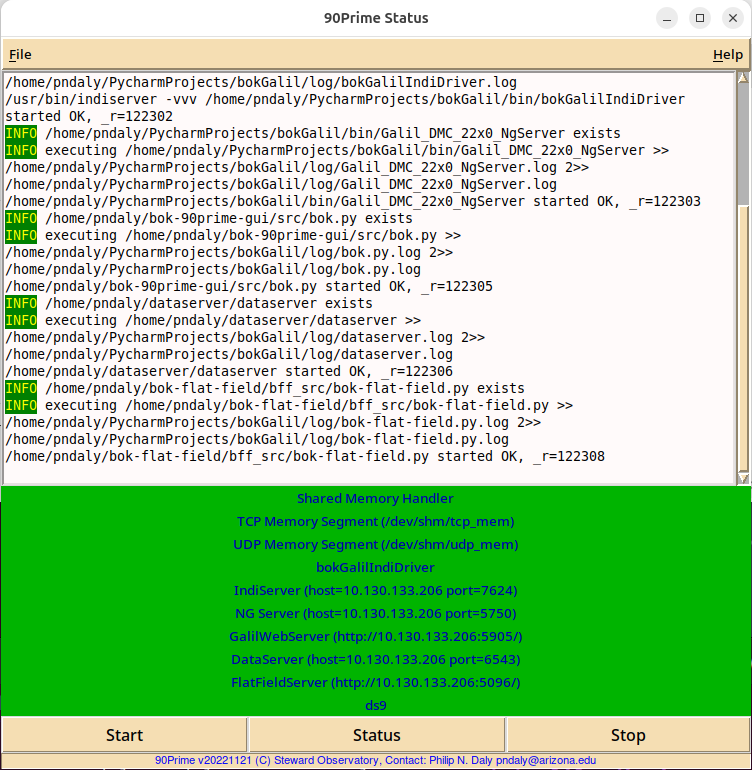
\includegraphics[width=0.4\linewidth]{bokSplashOn.png}
 \caption{The 90Prime Startup and Shutdown Interface.}
 \label{boktcl}
\end{figure}

\begin{figure}[!h]
 \centering
 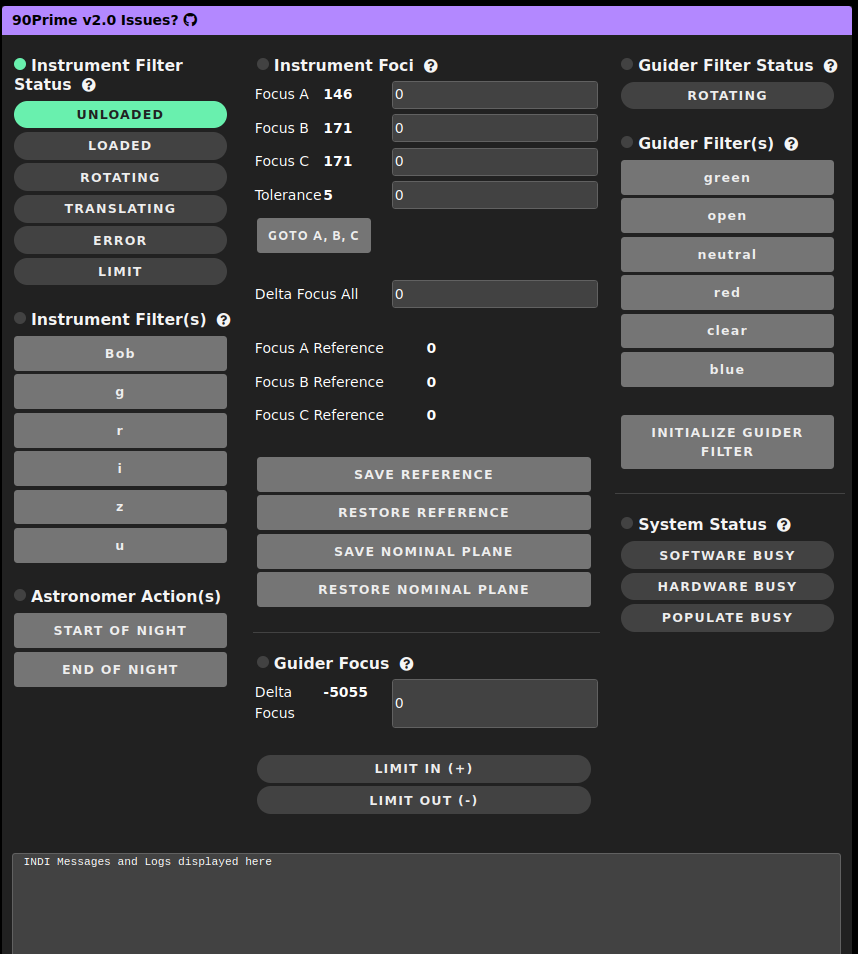
\includegraphics[width=0.5\linewidth]{AstronomerGUI.png}
 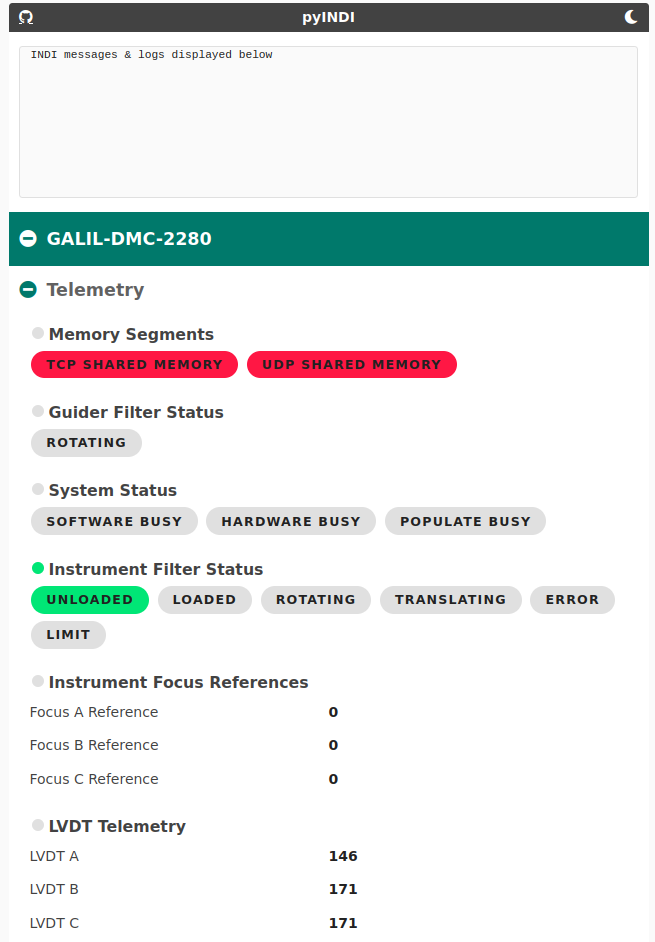
\includegraphics[width=0.4\linewidth]{EngineerGUI.png}
 \caption{The 90Prime Astronomer (left) and Engineer (right, only partially shown) GUIs.}
 \label{bokgui}
\end{figure}

\noindent To stop the system, press the \emteal{stop} button. The system status can be interrogated at any time by pressing 
the \emteal{status} button. Figure~\ref{boktcl} shows the system completely stopped on the left-hand side (all red) and
the system fully enabled on the right-hand side (all green). If any subsystem crashes, this interface will reflect the status
by changing that element from \emph{green} to \emph{red}. Note that the \emteal{start}, \emteal{stop} and \emteal{status} 
actions are global with no application to specific tasks. If a single task crashes, it is easiest to re-start the whole system
(and takes a few seconds at most).

\subsection{Filter File(s)}
\label{filterfiles}

\noindent The list(s) of available filters are stored in separate files in \$BOK\_GALIL\_DOCS:

\begin{description}
 \item[bok\_gfilters.txt] This file lists the available guider wheel filters;
 \item[bok\_ifilters.txt] This file lists the available instrument wheel filters and corresponds to the file in
                          /home/primefocus/90prime/galil/filters.txt on {\sc bart};
 \item[bok\_sfilters.txt] This file lists the available guider wheel filters and should be synchronized with 
                          bok\_gfilters.txt above.
\end{description}

\noindent These files can be edited as required. After editing, to check that the file(s) are usable by the system, execute: \\

\emteal{cd \$BOK\_GALIL\_BIN}

\emteal{./bok\_read\_filters -f\$BOK\_GALIL\_DOCS/bok\_gfilters.txt}

\emteal{./bok\_read\_filters -f\$BOK\_GALIL\_DOCS/bok\_ifilters.txt}

\emteal{./bok\_read\_filters -f\$BOK\_GALIL\_DOCS/bok\_sfilters.txt} \\

\noindent If these files are changed whilst the system is running, the system \emph{must} be re-started for them to take effect.

\subsection{/nfs/data/primefocus/\emph{yyyymmdd}}
\label{datadirectory}

A cronjob runs every day, just after local noon, to create a new data directory in /nfs/data/primefocus/\emph{yyyymmdd} where \emph{yyyymmdd} is the date at the start of the observing night (\emph{i.e. viz.,} local time). The observer or engineer will have to (manually) enter this directory in AzCam.

\subsubsection{Transferring Data Downtown}
\label{Transferring Data Downtown}

The \emph{primefocus} accounts on both \sfmagenta{bonsai} or \sfmagenta{banzai} have ssh-keys registered using the \emph{bok}
account on \sfmagenta{beast.as.arizona.edu}. Some command(s) to transfer this data are: \\
 
\emteal{ssh bokbeast mkdir data/yyyymmdd}

\emteal{ssh bokbeast chown -R bok:users data/yyyymmdd}

\emteal{rsync -avz /nfs/data/primefocus/yyyymmdd bokbeast:data/}

\emteal{ssh bokbeast chown -R bok:users data/yyyymmdd} \\

\noindent where \emph{yyyymmdd} is the observation date associated with the data directory shown in section~\ref{datadirectory} on page~\pageref{datadirectory}. The last 2 commands should be used regularly throughout the night.

\subsection{Day Crew Action(s)}
\label{daycrewactions}

\noindent When the software is started, the day crew will typically initialize the system via the following action(s)
accessed via the engineering interface (\ttblue{http://10.30.1.7:5905/indi}) as shown in Figure~\ref{engineer}):

\begin{description}
 \item[{\sc populate}] This command, once executed, allows the day crew to install various filters using the side 
                       button on the dewar;
 \item[{\sc populate done}] This command completes the populate filter wheel sequence;
 \item[{\sc initialize instrument filter}] This command reads the instrument filter wheel and must be allowed to complete;
 \item[{\sc initialize guider filter}] This (optional) command reads the guider filter wheel and, if invoked, must be allowed 
                                       to complete.
\end{description}

\begin{figure}[!h]
 \centering
 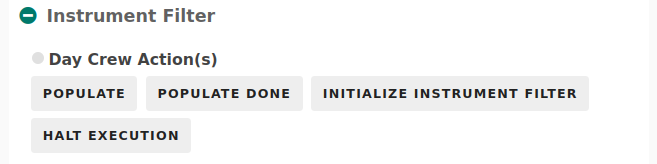
\includegraphics[width=0.5\linewidth]{DayCrewActions1.png}
 
\includegraphics[width=0.5\linewidth]{DayCrewActions2.png}
 \caption{The Day Crew Actions Within The Engineering GUI.}
 \label{engineer}
\end{figure}

\subsection{Running IRAF}
\label{Running IRAF}
Once the instrument is fully connected, day crew usually take an image to visually check the output array and check counts. This can be done
from {\sfmagenta bonsai} or {\sfmagenta banzai} by logging into the \emph{primefocus} account and executing: \\

\emteal{cd iraf\_docker}

\emteal{bash iraf yyyymmdd}

\noindent or

\emteal{bash iraf-community yyyymmdd} \\

where \emph{yyyymmdd} is the observation date associated with the data directory shown in section~\ref{datadirectory} on page~\pageref{datadirectory}. You will then have `ccdlist', `imexam' \emph{etc} available within the iraf window.

\subsection{Astronomer Night Action(s)}
\label{astronomernightactions}

\begin{description}
 \item[{\sc read filters}] This command reads the instrument filter wheel and must be allowed to complete. 
Do this at the start of every observing run or when the software is restarted;
 \item[{\sc load filter}] This command loads the currently selected instrument filter.
 \item[{\sc unload filter}] This command unloads any previously loaded instrument filter. 
It is good practice to unload the filter at the end of the observing night.
\end{description}

\subsection{Astronomer Flat Field Control}
\label{astronomerflatfieldcontrol}
Note that as part of the 90Prime startup, a new flat field GUI is created as shown in figure~\ref{bokff}. However, the
flat field controller in the computer rack must be manually turned on for these controls to become effective. The web
address for this GUI is \ttblue{http://10.30.1.7:5096} if running on \sfmagenta{bonsai} or \ttblue{http://10.30.1.8:5096} if running on \sfmagenta{banzai}.

\begin{figure}[!h]
 \centering
 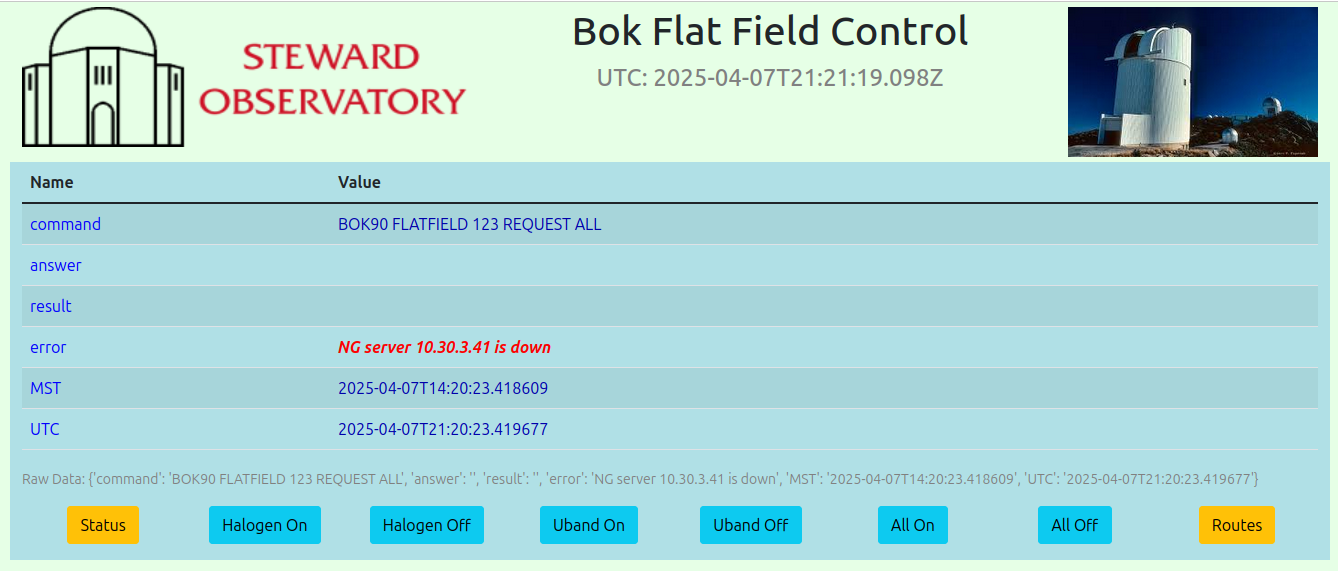
\includegraphics[width=0.8\linewidth]{bokFlatField.png}
 \caption{The Bok Flat Field Control Interface.}
 \label{bokff}
\end{figure}

\subsection{Astronomer Observer Log}
\label{astronomerobserverlog}

The directory \emteal{/home/primefocus/bok\_observer\_log} contains 2 utility programs that astronomers might find useful:

\begin{description}
 \item[\emteal{bok\_observer\_log.py}] This command produces a nightly observing log from the FITS header data within the specified path. It defaults to the observing night date in `yyyymmdd' format. An example of the output is show in figure~\ref{bokol}.
 \item[\emteal{bok\_observer\_fixfits.py}] This command is able to fix any FITS file header issues and add new keywords to the primary HDU only.
\end{description}

For the latter utility, there is a JSON-like syntax required by the code. As an example we can fix the OBSERVER keyword and add a new OBSCOMM keyword in the test.fits file like so:

\begin{verbatim}
    cd /home/primefocus/bok_observer_log
    python3 bok_observer_fixfits.py --file=test.fits \
        --data='{"OBSERVER": "Phil Daly", "OBSCOMM": "test comment"}'
\end{verbatim}

The OBSCOMM keyword is particularly useful since the bok\_observer\_log.py utility will pick it up and, if it's not 
empty, display it beneath the file in the output PDF. If in doubt, use the following commands to get some simple help:

\begin{verbatim}
    python3 bok_observer_log.py --help
    python3 bok_observer_fixfits.py --help
\end{verbatim}

\begin{figure}[!h]
 \centering
 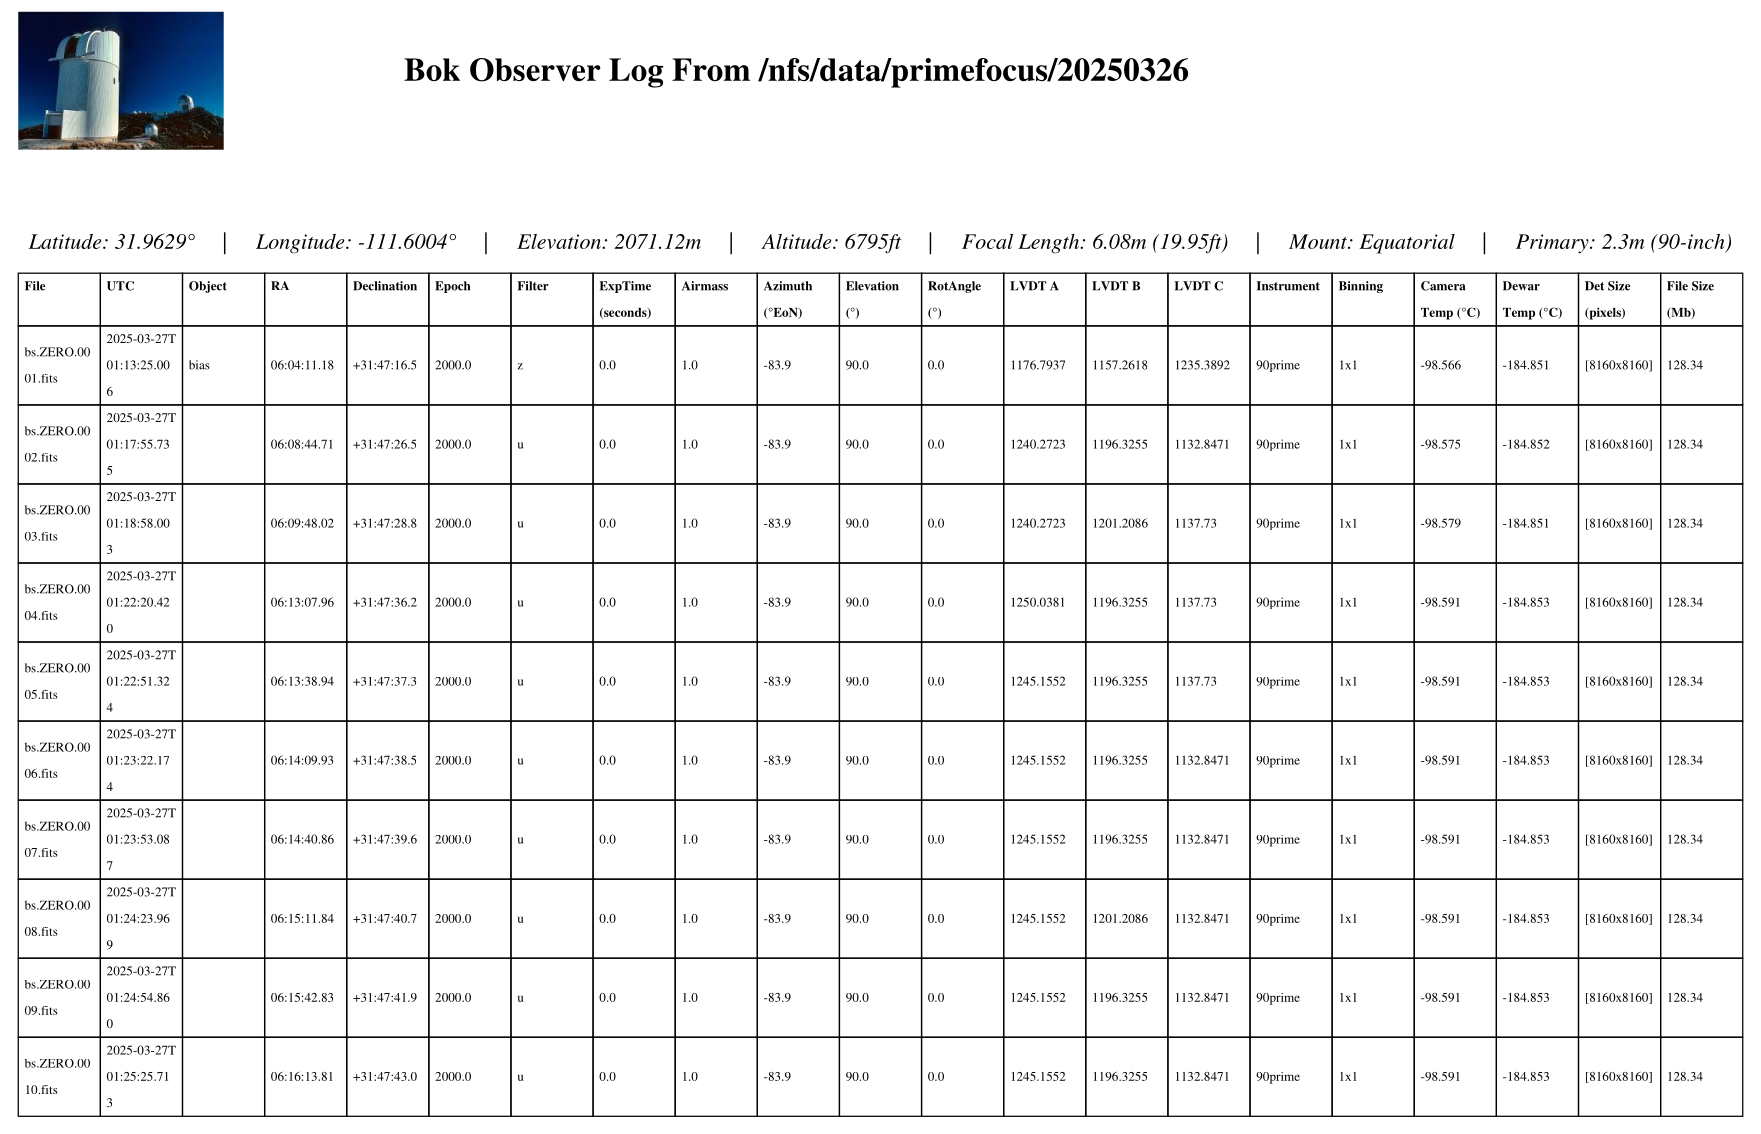
\includegraphics[width=0.8\linewidth]{bok_observer_log.png}
 \caption{The Bok Observer Log Output.}
 \label{bokol}
\end{figure}

\section{Emergency Shutdown}
\label{Emergency Shutdown}

Normally, the computer rack is \emph{always on} but there are times when an emergency shutdown is warranted. Even in this case, 
the KVM-switch (kvm), network switch (bokqnap) and UPS (bokups) are left powered up. The important hardware to shutdown cleanly 
are the NAS (\sfmagenta{boknas}) and 2 computers (\sfmagenta{bonsai}, \sfmagenta{banzai}). The following is the standard operating
procedure in this circumstance.

\subsection{Shutdown the NAS}
\begin{figure}[!h]
 \centering
 
\includegraphics[width=0.45\linewidth]{boknas1.png}
 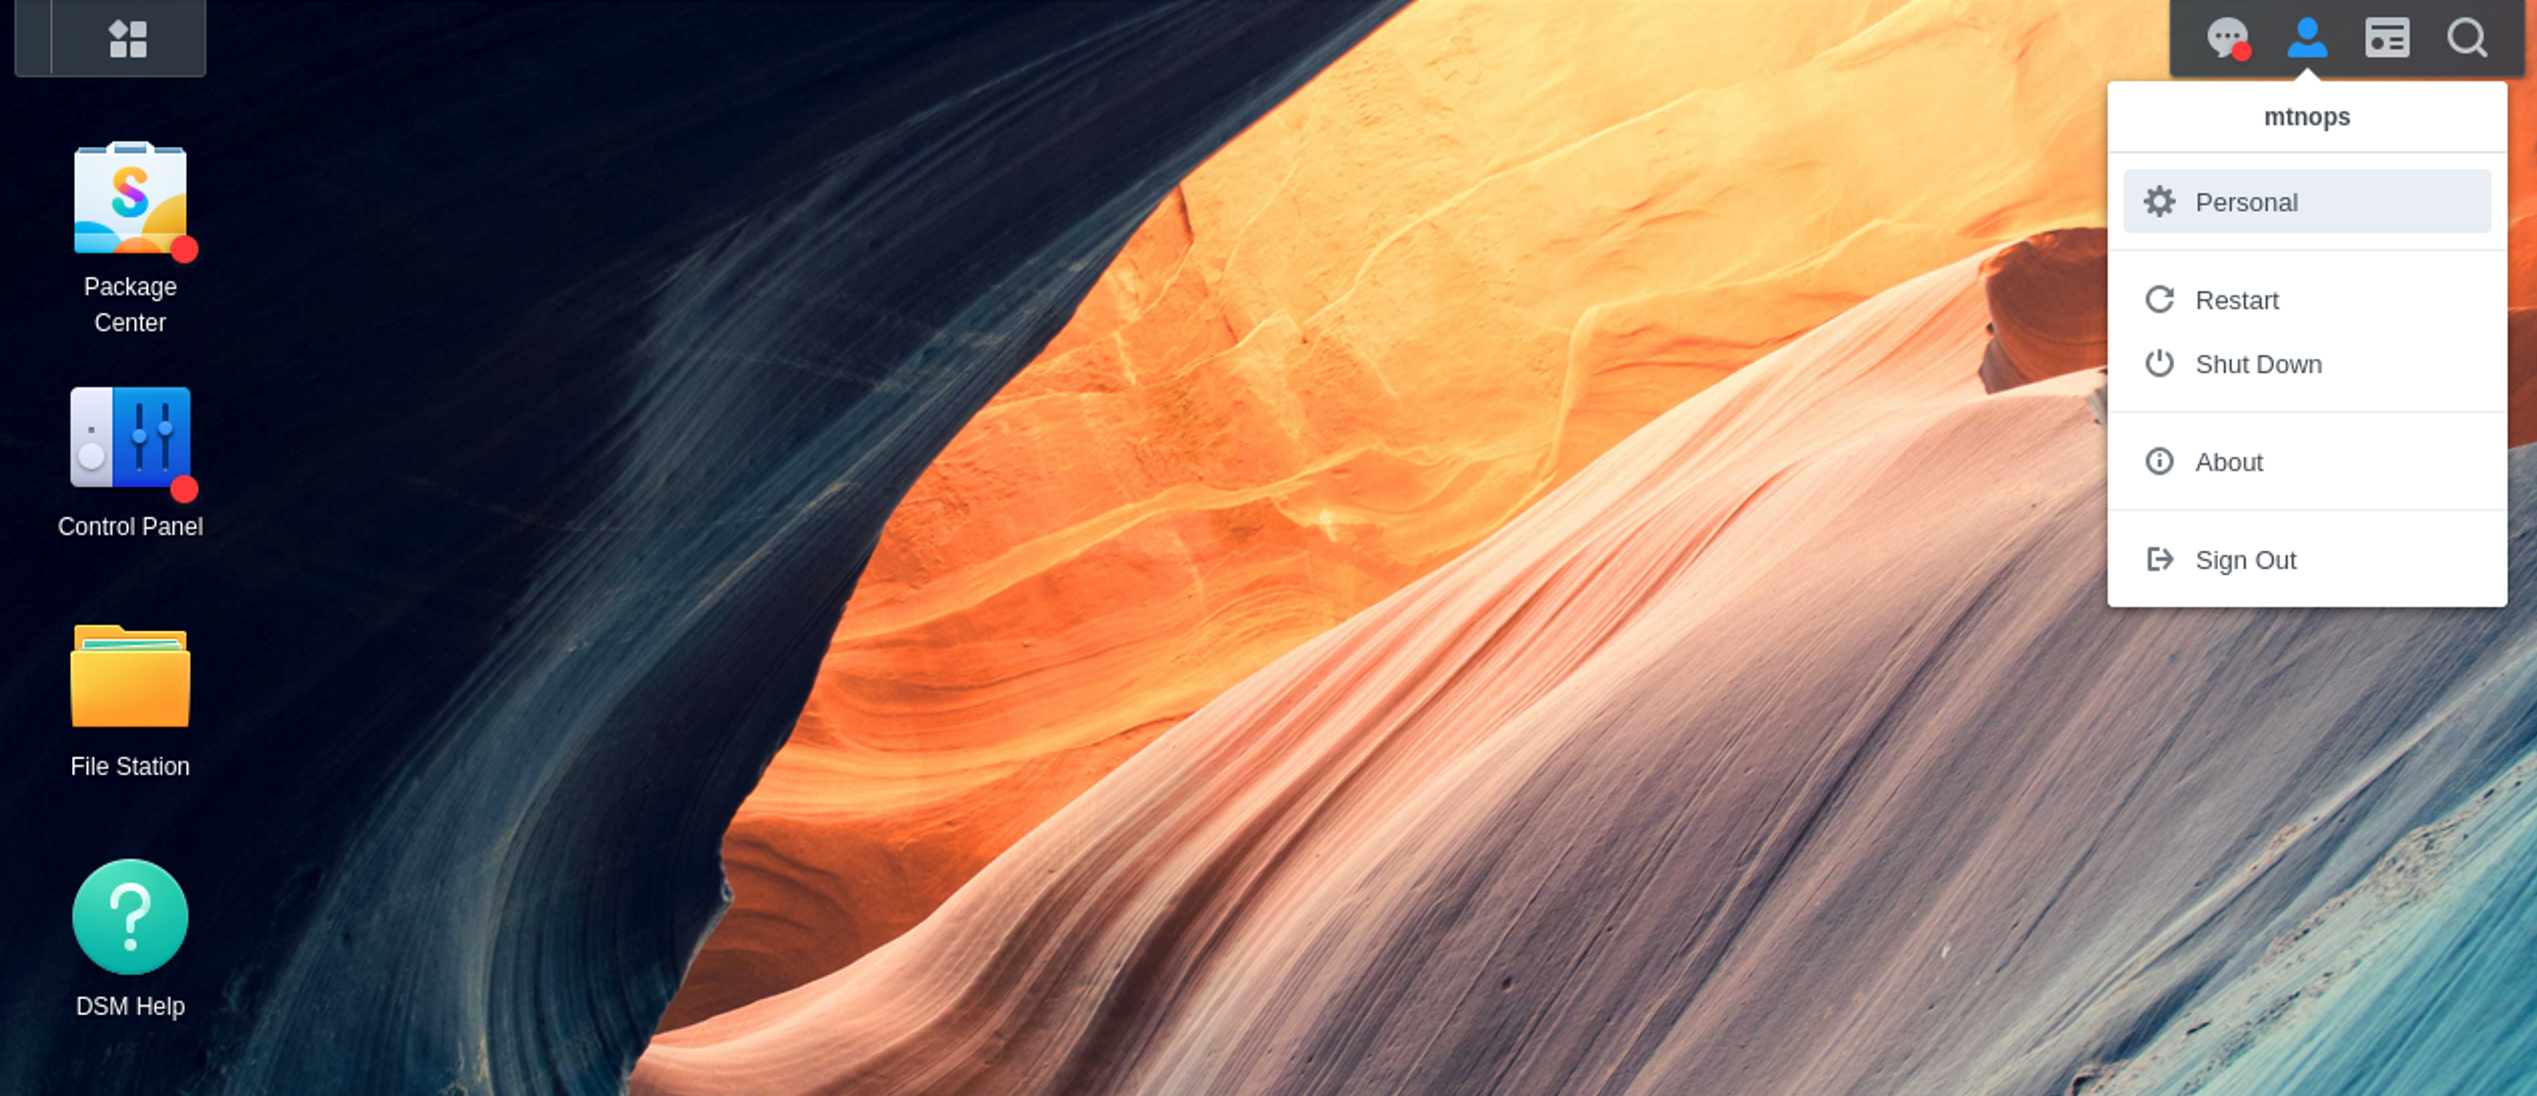
\includegraphics[width=0.45\linewidth]{boknas3.png}
 \caption{Shutting Down the NAS (\sfmagenta{boknas}).}
 \label{boknasshutdown}
\end{figure}

\begin{enumerate}
\item Login to either \sfmagenta{bonsai} or \sfmagenta{bonsai}.
\item Start a web-browser.
\item Navigate to http://10.30.1.9:5000 ... the screen should appear looking like the LHS of Figure~\ref{boknasshutdown}.
\item Login as \emph{mtnops} but the \emph{usual} password should have the `d' character capitalized to `D'!
\item The screen should change to looking like the RHS of Figure~\ref{boknasshutdown}.
\item Locate the person icon on the top right and click to see the drop-down menu.
\item Click on `Shut Down'.
\end{enumerate}

Allow a minute or two for the NAS to shutdown before proceeding to shutdown the computers.

\subsection{Shutdown the Computers}
\begin{figure}[!h]
 \centering
 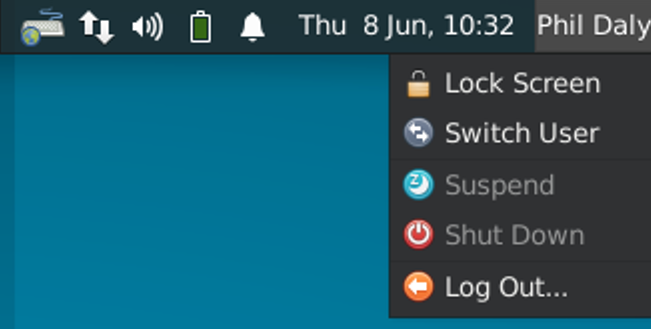
\includegraphics[width=0.45\linewidth]{bonsai1.png}
 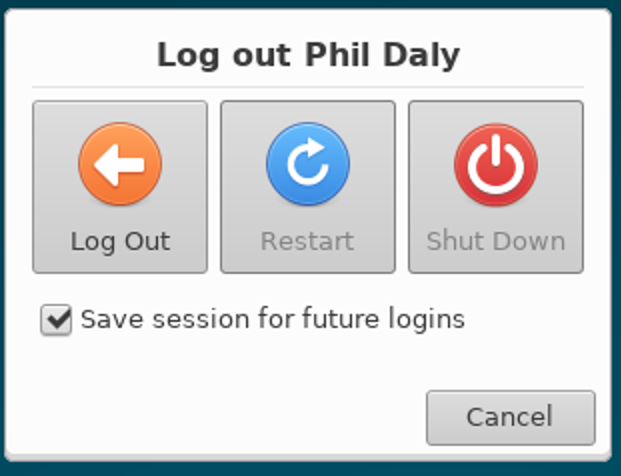
\includegraphics[width=0.45\linewidth]{bonsai2.png}
 \caption{Shutting Down the Computers (\sfmagenta{bonsai}, \sfmagenta{banzai}).}
 \label{computershutdown}
\end{figure}

The procedure for shutting down the computers is the same for both. Here we use \sfmagenta{bonsai} as the example.
The order is unimportant.

\begin{enumerate}
\item Login to either \sfmagenta{bonsai} as \emph{mtnops} with the usual password.
\item Click on the username (which should say `mtnops') in the top right of the screen to bring up the menu.
\item Click on `Shut Down'.
\item The pop-up window shown in Figure~\ref{computershutdown} should appear so click on `Shut Down'.
\item Repeat for \sfmagenta{banzai}.
\end{enumerate}

If you have difficulty using the GUI, a power off can be executed from the command line using `sudo poweroff'
(and you will be prompted for the mtnops password again).

\section{Hardware}
\label{Hardware}

\begin{figure}
 \centering
 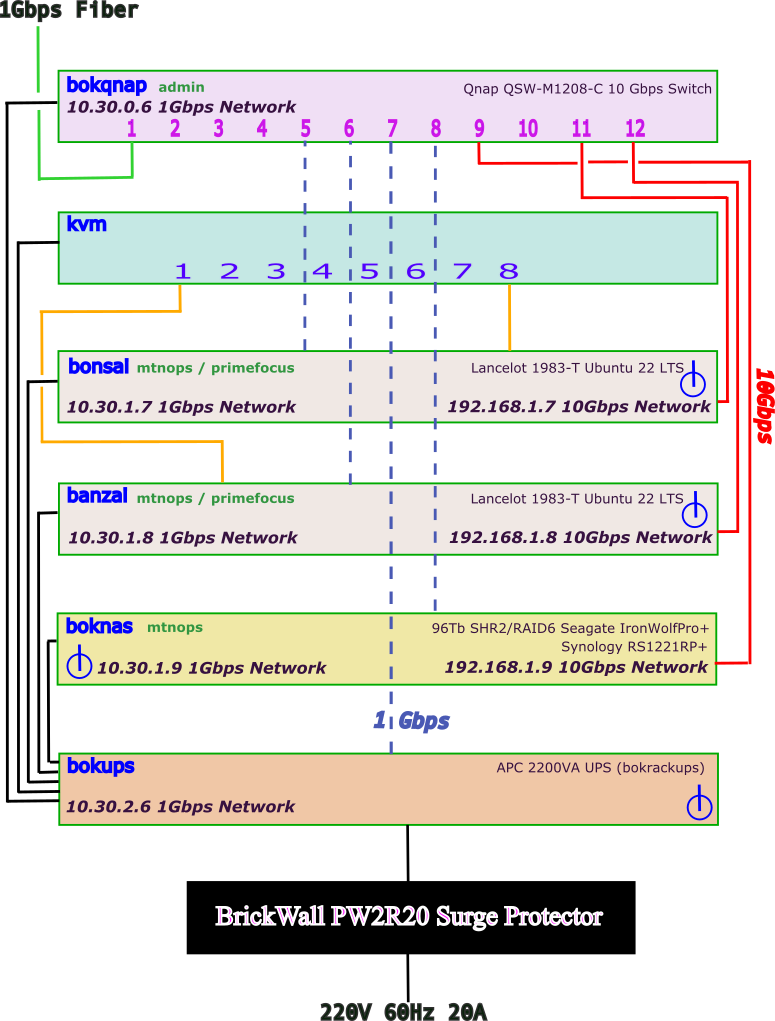
\includegraphics[angle=0,scale=0.75]{bokrack.png}
 \caption{The 90Prime System Rack.}
 \label{bokrack}
\end{figure}

\noindent A graphical representation of the hardware rack, installed in the 2$^{nd}$ floor office is shown in Figure~\ref{bokrack}.
The basic concept is for an {\sc always on} system that can withstand the usual Kitt Peak lightning activity so the
system is protected by a \emph{Brickwall} surge protector on a 20A circuit. The rack is further protected by an APC 
2200VA UPS. The CPU(s) are redundant inasmuch as, if \sfmagenta{bonsai} fails, \sfmagenta{banzai} can take over and vice-versa.
It is imperative, therefore, that infrastructure software on these machines is kept synchronized. We use GitHub repositories
for the Steward code base and well-documented procedures for obtaining the support software.

\begin{description}
\item[\sfmagenta{bonsai}] A Lancelot 1983-T 1U server from www.aslab.com. The specification is an
              Intel Xeon Silver 4210R 2.4GHz (10 cores), 6x8Gb DDR4-2933 Memory (48Gb),
              2 x Samsung 970 Evo Plus 2Tb SDD (RAID1), Intel X710-DA2 2-port PCIe x8 2 x SFP+ (10 Gbps),
              Ubuntu 20.04 LTS (ask for 22.x), 3 years support. The system was later upgraded to Ubuntu 22.04.2 LTS.
              This machine has a standard \emph{primefocus} account for running the software and a sudo-enabled \emph{mtnops}
              account for privileged actions.
              \sfmagenta{bonsai} is the primary \emph{data acquisition} system and \sfmagenta{banzai} the secondary.
\item[\sfmagenta{banzai}] A Lancelot 1983-T 1U server from www.aslab.com. The specification is an
              Intel Xeon Silver 4210R 2.4GHz (10 cores), 6x8Gb DDR4-2933 Memory (48Gb),
              2 x Samsung 970 Evo Plus 2Tb SDD (RAID1), Intel X710-DA2 2-port PCIe x8 2 x SFP+ (10 Gbps),
              Ubuntu 20.04 LTS (ask for 22.x), 3 years support. The system was later upgraded to Ubuntu 22.04.2 LTS.
              This machine has a standard \emph{primefocus} account for running the software and a sudo-enabled \emph{mtnops}
              account for privileged actions.
              \sfmagenta{banzai} is the primary \emph{data reduction} system and \sfmagenta{bonsai} the secondary.
\item[\sfmagenta{boknas}] A Synology RS1221RP$+$ chassis with 8x16Tb Seagate IronWolfPro$+$ mechanical drives. These are
              configured as a single 96Tb of SHR-2/RAID6 array NFS-mounted on \sfmagenta{bonsai} and \sfmagenta{banzai} as 
              /nfs/data. The Synology chassis was upgraded with (a total of) 32Gb of RAM and the E10M20-T1
              Ethernet / M2 combo card. This card supports the SNV3510-800 (800Gb) SSD cache and the 10Gbps
              network connection. The management account is \emph{mtnops} with the usual password but with the `d' capitalized!
              The management interface can be reached at \ttblue{http://10.30.1.9:5000/\#/signin/password}.
\item[\sfmagenta{bokqnap}] A QNAP QSW-M1208-C 10Gbps (dedicated and managed) Ethernet switch. The CPUs and NAS are attached
              via the 10 Gbps network for disk access and via the 1 Gbps network for regular network access. The management
              account is \emph{admin} with the standard \emph{mtnops} password. The management interface can be reached at
              \ttblue{http://10.30.0.6/\#/login}.
\item[\sfmagenta{bokups}] An APC 2200VA SMT2200RM2UC UPS that has enough capacity to support the whole rack. Note that this is
              attached to the network but has yet to be configured for automatic graceful shutdown after a given time has
              elapsed on battery power. Note that this may be referred to as \emph{bokrackups} in /etc/hosts.
\item[\sfmagenta{bokkvm}] An eKL VGA KVM Switch 8 Port 8x2 which supports Keyboard, Mouse, Audio, USB (although we use it in
              `dumb mode'). It has an IR remote control.
\end{description}

\section{Software}
\label{Software}

\begin{figure}
 \centering
 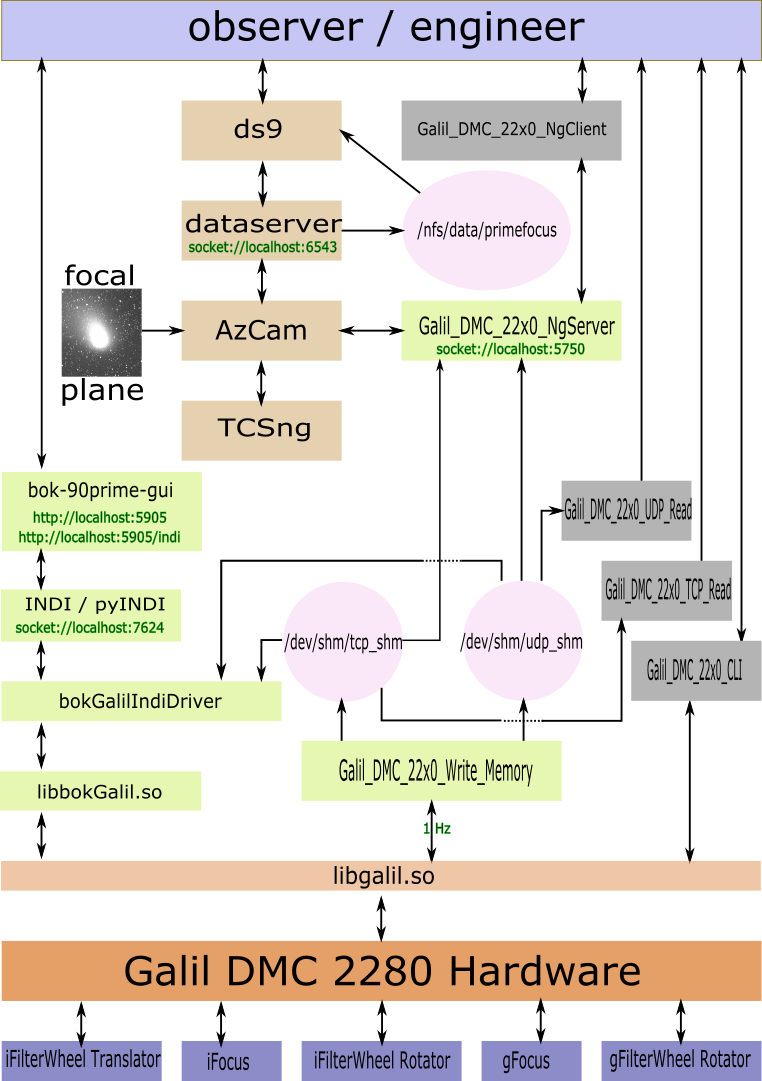
\includegraphics[angle=0,scale=0.75]{bokGalilIndiDriver.png}
 \caption{The 90Prime Software Architecture.}
 \label{bokGalilIndiDriver}
\end{figure}

The software is centered around the \emph{Instrument Neutral Distributed Interface}$^{\cite{1}, \cite{2}, \cite{3}}$
and the \emph{gclib} library provided by Galil$^{\cite{4}}$. An architecture diagram is shown in Figure~\ref{bokGalilIndiDriver}.
The software can built and run on any machine that supports the following:

\begin{itemize}
\item Ubuntu 22.04 LTS (or later)
\item INDI infrastructure code (www.indilib.org)
\item gclib (www.galil.com)
\item Python 3.8 (or later)
\item gcc 11.3.0 (or later)
\end{itemize}

\noindent Note that this software only supports /dev/shm shared memory under Unix.
Other repositories required to support operations are:

\begin{description}
\item[dataserver] \ttblue{https://github.com/so-mops/dataserver.git} \\
\item[bok-90prime-gui] \ttblue{https://github.com/so-90prime/bok-90prime-gui.git} \\
\item[pyINDI] \ttblue{https://github.com/MMTObservatory/pyINDI.git} \\
\end{description}

\subsection{Required Components}
\label{requiredcomponents}

In Figure~\ref{bokGalilIndiDriver} the minimum set of components required to run the system are:

\begin{description}
 \item[INDI / pyINDI] is the infrastructure software. The \emph{indiserver} can be installed following the instructions in
       Appendix~\ref{AppendixA}. The pyINDI software from the MMT is installed direct from a GitHub repository as part of
       the \emph{bok-90prime-gui} installation.
 \item[libgalil.so] This is the software library delivered by the vendor. It can be installed following the instructions in
       Appendix~\ref{AppendixB}.
 \item[libbokGalil.so] is the support library written by the author of this document to abstract the communications
      with the device.
 \item[bokGalilIndiDriver] is the INDI driver for the Galil.
 \item[Galil\_DMC\_22x0\_Write\_Memory] is an independent program running at 1 Hz that communicates with the 
       hardware and delivers key telemetry to shared memory segment(s) /dev/shm/tcp\_shm and /dev/shm/udp\_shm.
 \item[Galil\_DMC\_22x0\_NgServer] is an NG protocol server typically used by the AzCam software to retrieve data for FITS
      headers. The supported NG protocol commands and requests are documented in Appendix~\ref{AppendixC}.
\end{description}

\subsection{Optional Components}
\label{optionalcomponents}

\begin{description}
 \item[Galil\_DMC\_22x0\_NgClient] is \emph{not} required for normal operations but may be run to assist in debugging.
 \item[Galil\_DMC\_22x0\_CLI] is \emph{not} required for normal operations but may be run to assist in testing and debugging.
 \item[Galil\_DMC\_22x0\_TCP\_Read] is \emph{not} required for normal operations but may be run to assist in debugging.
 \item[Galil\_DMC\_22x0\_UDP\_Read] is \emph{not} required for normal operations but may be run to assist in debugging.
\end{description}

\subsection{Building The Software}
\label{buildingthesoftware}

\noindent The software can be installed directly from the GitHub repository. The following instructions assume that
the \emph{indiserver} has been built (see Appendix~\ref{AppendixA}) and \emph{gclib} installed (see Appendix~\ref{AppendixB}). \\

\emteal{git clone https://github.com/so-90prime/bokGalil.git}

\emteal{cd bokGalil}

\emteal{mkdir lib log}

\emteal{source etc/bokGalil.sh \$(pwd) load}

\emteal{cd \$BOK\_GALIL\_HOME}

\emteal{sudo python3 -m pip install -r requirements.txt}

\emteal{make -f ./test\_galil.make} \\

\noindent Note that \$BOK\_GALIL\_TCL/bokParams.bonsai.txt and \$BOK\_GALIL\_TCL/bokParams.banzai.txt should already exist 
but these should be checked for consistency with values reported in Table~\ref{variables}. Make the appropriate system: \\

\emteal{cd \$BOK\_GALIL\_TCL}

\emteal{make bonsai} \\

\noindent Note that \$BOK\_GALIL\_SRC/\_\_hosts\_\_.bonsai.h and \$BOK\_GALIL\_SRC/\_\_hosts\_\_.banzai.h should already exist 
but these should be checked for consistency with values reported in Table~\ref{variables}. The \_\_hosts\_\_.py file is 
automatically created. Make the appropriate system: \\

\emteal{cd \$BOK\_GALIL\_SRC}

\emteal{make bonsai} \\

\noindent Re-build this document (as required): \\

\emteal{cd \$BOK\_GALIL\_TEX}

\emteal{make all}

\subsection{Test}
\label{tests}

\subsubsection{test\_galil}

The easiest way to test the \emph{gclib} installation is to execute the test code: \\

\emteal{cd \$BOK\_GALIL\_HOME}

\emteal{./test\_galil -h} || \emteal{./test\_galil -b0} || \emteal{./test\_galil -b1} \\

\subsubsection{telnet}

A further test of the connectivity is to use the standard \emph{telnet} utility: \\

\emteal{telnet 10.30.3.31} \\

\noindent then execute the {\sc lv;} command. Data should appear. Use {\sc ctrl-]} to escape to the telnet prompt and 
enter {\sc quit}.

\subsubsection{XEphem}

Connect with XEphem $->$ View $->$ Sky View $->$ Telescope $->$ INDI panel $->$ Connect.

\subsubsection{Web Browser}

Connect either to the astronomer interface (\ttblue{http://10.30.1.7:5905}) or the engineering interface 
(\ttblue{http://10.30.1.7:5905/indi}) as shown in Figure~\ref{bokgui}.

\begin{landscape}
\begin{table}[h]
 \centering
 \caption{bokGalil Configuration Variable(s).}
 \label{variables}
 \begin{tabular}{llcc}
  \hline \hline
  & & & \\
  Variable & Description & \sfmagenta{bonsai} & \sfmagenta{banzai} \\
  & & & \\
  \hline
  & & & \\
  \_GALIL\_            & Galil DMC 2280 Hardware      & 192.168.0.100                    & 192.168.0.100                    \\
  BOK\_GALIL\_CMD\_BOK & Galil DMC 2280 Hardware      & 10.30.3.31                       & 10.30.3.31                       \\
  BOK\_GALIL\_CMD\_LAB & Galil DMC 2280 Spare         & 192.168.0.100                    & 192.168.0.100                    \\
  BOK\_INSTRUMENT      & Instrument                   & 90Prime                          & 90Prime                          \\
  BOK\_INDI\_ADDR      & IndiServer Address           & 10.30.1.7                        & 10.30.1.8                        \\
  BOK\_INDI\_PORT      & IndiServer Port              & 7624                             & 7624                             \\
  BOK\_NG\_ADDR        & NG Server Address            & 10.30.1.7                        & 10.30.1.8                        \\
  BOK\_NG\_PORT        & NG Server Port               & 5750                             & 5750                             \\
  BOK\_TCP\_ADDR       & Galil TCP Command Address    & 10.30.3.31                       & 10.30.3.31                       \\
  BOK\_TCP\_PORT       & Galil TCP Command Port       & 23                               & 23                               \\
  BOK\_UDP\_ADDR       & Galil UDP Command Address    & 10.30.1.7                        & 10.30.1.8                        \\
  BOK\_UDP\_PORT       & Galil UDP Command Port       & 5078                             & 5078                             \\
  BOK\_WEB\_ADDR       & pyINDI Website Address       & 10.30.1.7                        & 10.30.1.8                        \\
  BOK\_WEB\_PORT       & pyINDI Website Port          & 5905                             & 5905                             \\
  BOK\_WEB\_REPO       & pyINDI Website Repository    & /home/primefocus/bok-90prime-gui & /home/primefocus/bok-90prime-gui \\
  BOK\_DATA\_ADDR      & DataServer Address           & 10.30.1.7                        & 10.30.1.8                        \\
  BOK\_DATA\_PORT      & DataServer Port              & 6543                             & 6543                             \\
  BOK\_DATA\_REPO      & DataServer Repository        & /home/primefocus/dataserver      & /home/primefocus/dataserver      \\
  BOK\_FF\_REPO        & FlatField Website Repository & /home/primefocus/bok-flat-field  & /home/primefocus/bok-flat-field  \\
  BOK\_FF\_ADDR        & FlatField Website Address    & 10.30.1.7                        & 10.30.1.8                        \\
  BOK\_FF\_PORT        & FlatField Website Port       & 5096                             & 5096                             \\
  & & & \\
  \hline \hline
 \end{tabular}
\end{table}
\end{landscape}

\subsection{Debugging}
\label{Debugging}
Log files are written to \$BOK\_GALIL\_LOG. The Galil\_DMC\_22x0\_CLI interface may also be run: at the command prompt enter `?'
for options. Any Galil supported command may be sent to the hardware if the Galil\_DMC\_22x0\_CLI program is invoked with the
\emph{-o} (override) option!

\begin{thebibliography}
 \bibitem{1} [1] https://en.wikipedia.org/wiki/Instrument\_Neutral\_Distributed\_Interface.
 \bibitem{2} [2] https://www.indilib.org.
 \bibitem{3} [3] http://www.clearskyinstitute.com/INDI/INDI.pdf.
 \bibitem{4} [4] https://www.galil.com/sw/pub/all/doc/gclib/html/ubuntu.html.
\end{thebibliography}

\appendix
\newpage
\section{INDI Installation}
\label{AppendixA}

Execute the following commands (as root): \\

\emteal{apt update}

\emteal{apt-get install -y git cdbs dkms cmake swig fxload libev-dev libgps-dev libgsl-dev libraw-dev}

\emteal{apt-get install -y libusb-dev zlib1g-dev libftdi-dev libgsl0-dev libjpeg-dev libkrb5-dev}

\emteal{apt-get install -y libnova-dev libtiff-dev libfftw3-dev librtlsdr-dev libcfitsio-dev}

\emteal{apt-get install -y libgphoto2-dev build-essential libusb-1.0-0-dev libdc1394-dev}

\emteal{apt-get install -y libboost-regex-dev libcurl4-gnutls-dev libtheora-dev libxml2-utils} \\

\noindent Build the software (as root): \\

\emteal{rm -rf /usr/local/IndiProjects}

\emteal{mkdir -p /usr/local/IndiProjects}

\emteal{cd /usr/local/IndiProjects}

\emteal{git clone https://github.com/indilib/indi.git}

\emteal{mkdir -p /usr/local/IndiProjects/build/indi-core}

\emteal{cd /usr/local/IndiProjects/build/indi-core}

%%\emteal{cmake -DCMAKE\_INSTALL\_PREFIX=/usr -DCMAKE\_BUILD\_TYPE=Debug /usr/local/IndiProjects/indi}
\emteal{cmake -DCMAKE\_BUILD\_TYPE=Debug /usr/local/IndiProjects/indi}

\emteal{make -j4}

\emteal{make install} \\

\noindent Optionally, install the Python client (as root): \\

\emteal{apt-get install -y python3-pip}

\emteal{python3 -m pip install --upgrade pip}

\emteal{python3 -m pip install pyindi-client}

\section{gclib Installation}
\label{AppendixB}

Execute the following commands (as root). First, get and install the key: \\

\emteal{wget https://www.galil.com/sw/pub/all/crypto/GALIL-GPG-KEY-E29D0E4B.asc}

\emteal{mv GALIL-GPG-KEY-E29D0E4B.asc /etc/apt/trusted.gpg.d/} \\

\noindent Second, update the repository list: \\

\emteal{curl -O https://www.galil.com/sw/pub/ubuntu/22.04/galil.list}

\emteal{mv galil.list /etc/apt/sources.list.d/} \\

\noindent Finally, install the software: \\

\emteal{apt update}

\emteal{apt remove gclib gcapsd}

\emteal{apt install gclib gcapsd}

\newpage
\section{NG Protocol Commands and Requests}
\label{AppendixC}

The software supports the standard NG protocol syntax: \\

\ttblue{$<$telescope$>$ $<$instrument$>$ $<$cmd-id$>$ $<$COMMAND||REQUEST$>$ $<$extra-information$>$} \\

\noindent If $<$cmd-id$>$ is set to {\sc simulate}, no hardware is accessed and dummy response(s) are returned!
Commands and requests are case insensitive. \\

\noindent All \emph{commands}, return one of the following responses:

 \begin{description}
  \item[On success] bok 90prime $<$cmd-id$>$ OK
  \item[On failure] bok 90prime $<$cmd-id$>$ ERROR $<$reason$>$
 \end{description}

\noindent All \emph{requests}, return one of the following responses:

 \begin{description}
  \item[On success] bok 90prime $<$cmd-id$>$ OK $<$returned-data-values$>$
  \item[On failure] bok 90prime $<$cmd-id$>$ ERROR $<$reason$>$
 \end{description}

\subsection{Supported Command(s)}

\subsubsection{bok 90prime $<$cmd-id$>$ command exit}
  --- client informs server it's shutting down.

\subsubsection{bok 90prime $<$cmd-id$>$ command gfilter init}
  --- client commands server to initialize guider filter wheel.
 
\subsubsection{bok 90prime $<$cmd-id$>$ command gfilter name $<$str$>$}
  --- client commands server to change guider filter to given name.
 
\subsubsection{bok 90prime $<$cmd-id$>$ command gfilter number $<$int$>$}
  --- client commands server to change guider filter to given number.
 
\subsubsection{bok 90prime $<$cmd-id$>$ command gfocus delta $<$float$>$}
  --- client commands server to change guider focus to given value.

\subsubsection{bok 90prime $<$cmd-id$>$ command ifilter init}
  --- client commands server to initialize instrument filter wheel.

\subsubsection{bok 90prime $<$cmd-id$>$ command ifilter name $<$str$>$}
  --- client commands server to change instrument filter to given name.

\subsubsection{bok 90prime $<$cmd-id$>$ command ifilter number $<$int$>$}
  --- client commands server to change instrument filter to given number.
 
\subsubsection{bok 90prime $<$cmd-id$>$ command ifilter load}
  --- client commands server to insert current filter into beam.

\subsubsection{bok 90prime $<$cmd-id$>$ command ifilter unload}
  --- client commands server to remove current filter from beam.

\subsubsection{bok 90prime $<$cmd-id$>$ command ifocus a $<$float$>$ b $<$float$>$ c $<$float$>$ t $<$float$>$}
  --- client commands server to change instrument focus in all 3 axes by separate amounts within tolerance.

\subsubsection{bok 90prime $<$cmd-id$>$ command ifocusall delta $<$float$>$ t $<$float$>$}
  --- client commands server to change instrument focus in all 3 axes by the same amount within tolerance

\subsubsection{bok 90prime $<$cmd-id$>$ command lvdt a $<$float$>$ b $<$float$>$ c $<$float$>$ t $<$float$>$}
  --- client commands server to change instrument LVDTs in all 3 axes by separate amounts within tolerance.

\subsubsection{bok 90prime $<$cmd-id$>$ command lvdtall $<$float$>$ t $<$float$>$}
  --- client commands server to change instrument LVDTs in all 3 axes by the same amount within tolerance.
 
\subsubsection{bok 90prime $<$cmd-id$>$ command test}
  --- client commands server to test communication path.
 
\subsubsection{bok 90prime $<$cmd-id$>$ command hx}
  --- client commands server to halt execution in the galil controller.
 
\subsection{Supported Request(s)}

\subsubsection{bok 90prime $<$cmd-id$>$ request encoders}
  --- client requests encoder values. An example response might be `{\sc bok 90prime $<$cmd-id$>$ ok a=-0.355 b=1.443 c=0.345}'.

\subsubsection{bok 90prime $<$cmd-id$>$ request gfilter}
  --- client requests server to report current guider filter. An example response might be `{\sc bok 90prime $<$cmd-id$>$ ok gfiltn=4:red rotating=false}'.

\subsubsection{bok 90prime $<$cmd-id$>$ request gfilters}
  --- client requests server to report guider filters. An example response might be `{\sc bok 90prime $<$cmd-id$>$ ok 1=1:green 2=2:open 3=3:neutral 4=4:red 5=5:open 6=6:blue}'.

\subsubsection{bok 90prime $<$cmd-id$>$ request gfocus}
  --- client requests server to report guider focus. An example response might be `{\sc bok 90prime $<$cmd-id$>$ ok gfocus=-0.355}'.

\subsubsection{bok 90prime $<$cmd-id$>$ request ifilter}
  --- client requests server to report current instrument filter. An example response might be `{\sc bok 90prime $<$cmd-id$>$ ok filtval=18:bob inbeam=true rotating=false translating=false errfilt=0 filttsc=3}'.

\subsubsection{bok 90prime $<$cmd-id$>$ request ifilters}
  --- client requests server to report instrument filters. An example response might be `{\sc bok 90prime $<$cmd-id$>$ ok 0=18:Bob 1=2:g 2=3:r 3=4:i 4=5:z 5=6:u}'.

\subsubsection{bok 90prime $<$cmd-id$>$ request ifocus}
  --- client requests server to report instrument focus. An example response might be `{\sc bok 90prime $<$cmd-id$>$ ok a=-0.355 b=1.443 c=0.345}'.

\end{document}
